\section{Sensitivity of LHC measurements to Vector-like Quarks}
\label{sec:VLQ}
Vector-like quarks belong to a separate family than the SM quarks. They are non-chiral, and thus both the left- and right-handed components transofrm the same way under the SM symmetries. This enables them to have a bare mass term and obtain mass without interacting with the Higg boson. Consequently, they are not constrained by Higgs measurements, unlike a fourth generation in the SM quark family. In short, VLQs are simplest example of coloured fermions still allowed by experimental data \cite{Aguilar_Saavedra_2013}. 

Vector-like quarks arise in many classes of BSM theories, such as composite Higgs that assume electroweak symmetry breaking is due to a a new strongly interacting sector~\cite{witzel2019review}, or little Higgs models that introduce extended global symmetries, or models with extra dimensional symmetries \todo{Add some citations for these models}. As with most models extending the SM, many of these introduce new sources of CP violation.

\subsection{Phenomenology of VLQs}
For the material presented in this section, vector-like quarks are studied in a model-independent fashion involving few free parameters. The framework is developed in Reference~\cite{}, which presents an effective Lagrangian description for vector-like quarks that is easily translated to experimental observables. The Lagrangian is written in equation 3.2 of Reference~\cite{} as:
\begin{equation}
  \label{eq:vlqlagr}
  \begin{split}
    \mathcal{L} =
    &  \kappa_B \left[
      \sqrt{\frac{\zeta_i\xi^{B}_{W}}{\Gamma^0_{W}}} \frac{g}{\sqrt{2}} [\bar{B}_{L/R} W^-_\mu \gamma^\mu u^i_{L/R}]
      +  \sqrt{\frac{\zeta_i\xi^{B}_{Z}}{\Gamma^0_{Z}}} \frac{g}{2c_W} [\bar{B}_{L/R} Z_\mu \gamma^\mu d^{\,i}_{L/R}]
      -  \sqrt{\frac{\zeta_i\xi^{B}_{H}}{\Gamma^0_{H}}} \frac{M_B}{v} [\bar{B}_{R/L} H d^{\,i}_{L/R}]
    \right] \\
    + &   \kappa_T \left[
      \sqrt{\frac{\zeta_i\xi^{T}_{W}}{\Gamma^0_{W}}} \frac{g}{\sqrt{2}} [\bar{T}_{L/R} W^+_\mu \gamma^\mu d^{\,i}_{L/R}]
      +  \sqrt{\frac{\zeta_i\xi^{T}_{Z}}{\Gamma^0_{Z}}} \frac{g}{2c_W} [\bar{T}_{L/R} Z_\mu \gamma^\mu u^i_{L/R}]
      -  \sqrt{\frac{\zeta_i\xi^{T}_{H}}{\Gamma^0_{H}}} \frac{M_T}{v} [\bar{T}_{R/L} H u^i_{L/R}]
    \right] \\
    +  &  \kappa_X \left[
      \sqrt{\frac{\zeta_i}{\Gamma^0_{W}}} \frac{g}{\sqrt{2}} [\bar{X}_{L/R} W^+_\mu \gamma^\mu u^i_{L/R}]
    \right]
    + \kappa_Y \left[
      \sqrt{\frac{\zeta_i}{\Gamma^0_{W}}} \frac{g}{\sqrt{2}} [\bar{Y}_{L/R} W^-_\mu \gamma^\mu d^{\,i}_{L/R}]
    \right] + \text{h.c.} \, ,
    % + & \kappa_g \left[ \frac{g_s v}{2\Lambda^2} f_i^{L/R} \bar{Q}_{R/L} G_{\mu\nu}\sigma^{\mu\nu} q^{i}_{L/R} \right] + h.c...
  \end{split}
\end{equation}
where $B$, $T$, $X$, and $Y$ are the four types of vector-like quarks with triplet colour charges, and electromagnetic charges $-\frac{1}{3}$, $\frac{2}{3}$, $\frac{5}{3}$ and $-\frac{4}{3}$ respectively. The couplings with the photon and gluon are derived via the standard gauge invariance route. The overall coupling strength of the vector-like quarks $Q$ are governed by the parameters $\kappa_Q$. $\zeta_i$ represents the coupling of the vector-like quarks to the $i^\text{th}$ generation SM quark. $\xi^B_V$ and $\xi^T_V$ govern the couplings of the $B$ and $T$ quarks to $Z$, $W$, and Higgs bosons via new $QqV$ vertices. Another free parameter is the mass of the new quarks, denoted as $M_Q$. Under the assumption that $\sum_{V} \xi^B_{V} = 1$ and $\sum_{V} \xi^T_{V} = 1$, and $\sum_{i} \zeta_i = 1$, the branching ratio of any vector-like quark to an SM quark and gauge boson is written as
\begin{equation}
    \textrm{BR}(Q \rightarrow Vq_i) = \zeta_i\xi^{V}.
\end{equation}

At the LHC, vector-like quarks can be either pair- or singly-produced. Pair-production occurs via the strong and electromagnetic interaction, and via the weak interaction through the $t$-channel exchange of an SM weak boson. Single production in association with a quark or with an SM boson occurs via the weak interaction only. Examples of leading-order Feynman diagrams for VLQ production are shown in Figure~\ref{fig:feyndiags}. Vector-like quarks can only decay via the weak interaction into an SM weak boson and an SM quark. Given the charge assignments, the possible decay channels of the vector-like quarks are:
\begin{equation}
    B^{-\frac{1}{3}}\rightarrow W^- + q_u, \quad Z + q_d, \quad H + q_d \\
    T^{+\frac{2}{3}}\rightarrow W^+ + q_d, \quad Z + q_u, \quad H + q_u \\
    X^{+\frac{5}{3}}\rightarrow W^+ + q_u \\
    Y^{-\frac{4}{3}}\rightarrow W^- + q_d .
\end{equation}
The $B$ and $T$ quark decays to the $W$, $Z$, or Higgs boson plus an up- or down-type quark, depending on the values of the $\xi^V$ and $\zeta_i$ parameters. The $X$ and $Y$ quarks, however, can only decay via the $W$ decay channel due to electromagnetic charge conservation, and are unaffected by the values of $\xi^V$\footnote{Since $\xi^W$=1 and $\xi^Z=\xi^H=0$ are constants for $X$ and $Y$.}. The production rates of the vector-like quarks depend on the mass $m_Q$, especially for the QCD-dominated pair production~\cite{Buchkremer_2013}. The coupling strength factors $\kappa_Q$ drive the electroweak production cross-sections, which are therefore sensitive to the overall strength of the coupling.
\begin{figure}[t]
  \centering
  \subfloat[]{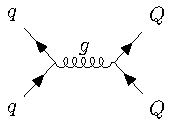
\includegraphics[]{Figures/VLQ/feynmanDiagrams/diagram-5.pdf}\label{fig:feyndiags:QQ1}}
  \subfloat[]{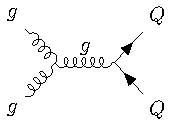
\includegraphics[]{Figures/VLQ/feynmanDiagrams/diagram-9.pdf}\label{fig:feyndiags:QQ2}}
  \subfloat[]{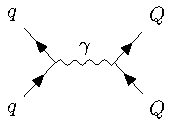
\includegraphics[]{Figures/VLQ/feynmanDiagrams/diagram-6.pdf}\label{fig:feyndiags:QQ3}}\\
  \subfloat[]{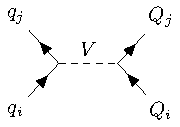
\includegraphics[]{Figures/VLQ/feynmanDiagrams/diagram-8.pdf}\label{fig:feyndiags:QQ'1}}
  \subfloat[]{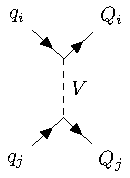
\includegraphics[]{Figures/VLQ/feynmanDiagrams/diagram-7.pdf}\label{fig:feyndiags:QQ'2}}\\
  \subfloat[]{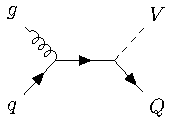
\includegraphics[]{Figures/VLQ/feynmanDiagrams/diagram-1.pdf}\label{fig:feyndiags:QV1}}
  \subfloat[]{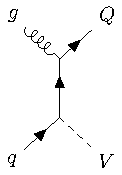
\includegraphics[]{Figures/VLQ/feynmanDiagrams/diagram-2.pdf}\label{fig:feyndiags:QV2}}
  \subfloat[]{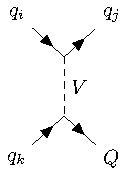
\includegraphics[]{Figures/VLQ/feynmanDiagrams/diagram-3.pdf}\label{fig:feyndiags:Qq1}}
  \subfloat[]{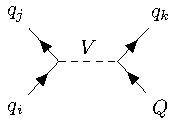
\includegraphics[]{Figures/VLQ/feynmanDiagrams/diagram-4.pdf}\label{fig:feyndiags:Qq2}}
  \caption{Leading-order Feynman diagrams for production of VLQs $Q$.  The top row (\protect\subref*{fig:feyndiags:QQ1}--\protect\subref*{fig:feyndiags:QQ3}) shows VLQ pair-production diagrams via strong and EM interactions, which do not depend on $\kappa$.  The second row (\protect\subref*{fig:feyndiags:QQ'1}--\protect\subref*{fig:feyndiags:QQ'2}) shows pair-production of VLQs via a weak boson $V \in \{W,Z,H\}$, which may lead to different-flavoured VLQs in the final state. The third row (\protect\subref*{fig:feyndiags:QV1}--\protect\subref*{fig:feyndiags:Qq2}) shows single-production of $Q$ in association with a weak boson or SM quark $q$. All Feynman diagrams are taken from Reference~\cite{VLQ_contur}}.
\label{fig:feyndiags}
\end{figure}

The phenomenology of vector-like quark production and decay can be inferred from the Lagrangian of Equation~\ref{eq:vlqlagr}. In particular, the production cross-sections are dependent on $M_Q$ and $\kappa$. For this section, it is assumed that the $B,T,X$, and$Y$ quarks all have the same mass and coupling strength (i.e. $M_B = M_T = M_X = M_Y$ and $\kappa_B = \kappa_T = \kappa_X = \kappa_Y$). 

\subsubsection{Pair production}

Figures~\ref{fig:feyndiags}(\subref*{fig:feyndiags:QQ1}--\subref*{fig:feyndiags:QQ3}) show the pair production of VLQs via the strong and electromagnetic interaction. These three diagrams are not dependent on any of the coupling parameters $\kappa,\xi$ or $\zeta$. For a VLQ of mass
$\sim \unit{1.3}{\TeV}$ at the LHC, the cross-section is of the order of $\unit{10}{\femto\barn}$~\cite{VLQ_contur}. In the second row, Figures~\ref{fig:feyndiags}(\subref*{fig:feyndiags:QQ'1}--\subref*{fig:feyndiags:QQ'2}) show the s- and t-channel pair-production of VLQs through the exchange of a weak boson. These diagrams are dependent on $\kappa$, and may have a non-negligible contribution to the production cross-section. In fact, when the VLQs couple only to first generation SM quarks, Figure~\ref{fig:feyndiags:QQ'2} can become the dominant production mechanism. Since the up and down quarks are the constituents of the proton, Figure~\ref{fig:feyndiags:QQ'2} is the only possible diagram with two incoming valence quarks. All other diagrams require at least one anti-quark or gluon. If the VLQs couple to the second or third generation SM quarks, however, Figure~\ref{fig:feyndiags:QQ'2} is no longer dominant. This effect is illustrated in Figure~\ref{fig:TTproduction} for $TT$ pair-production. For VLQs coupling to the first generation, a dependence on $\kappa$ becomes visible as the mass of the VLQs increase. This feature is not visible for couplings to the second and third generation. The VLQs are produced in pairs of different flavours when mediated by a $W$ boson. For the $X$ and $Y$, this is always the case since they do not couple to the $Z$ or the Higgs. 
\begin{figure}[tbp]
\vspace{-0.4cm}
\subfloat[$T$ coupling to $u,d$ only]{\includegraphics[width=0.33\textwidth]{xsScans/1stGen/p_p____T_T.pdf}} %5000 fb
\subfloat[$T$ coupling to $c,s$ only]{\includegraphics[width=0.33\textwidth]{xsScans/2ndGen/p_p____T_T.pdf}} %5000 fb\\
\subfloat[$T$ coupling to $t,b$ only]{\includegraphics[width=0.33\textwidth]{xsScans/3rdGen/p_p____T_T.pdf}}
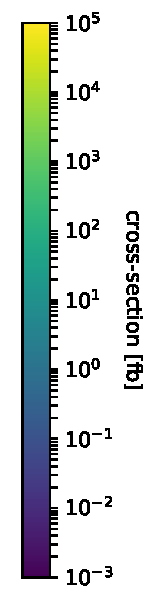
\includegraphics[height=3.5cm]{xsScans/3rdGen/cbar.pdf} %5000 fb
\caption{Leading-order cross-sections extracted from Herwig for production of a $TT$ pair as a
  function of $M_Q$ and $\kappa$, for \unit{13}{\TeV} $pp$ collisions, in the
  $\WZH = \WZHtoo$ scenario, assuming couplings to individual generations of
  quarks.  The white lines indicate the contours for production cross-sections
  in multiples of 10. The first-generation cross-sections acquire a dependence
  on $\kappa$ since pair-production initiated by proton valence quarks becomes
  possible.  The situation is analogous for other VLQ flavours, although
  somewhat attenuated for $X$ and $Y$ since they still require at least one
  antiquark from the sea to be produced via $W$ exchange in the $t$-channel. Figure taken from Reference~\cite{VLQ_contur}.}
\label{fig:TTproduction}
\end{figure}

\subsubsection{Single production}
Single production is illustrated in the last row of Figure~\ref{fig:feyndiags}. It can occur in association with a weak boson $V$, or with a Standard Model quark $q$. In both cases a strong $\kappa$ dependence is present since single production always takes place via the weak interaction. 

Looking first at VLQ production alongside a weak boson, it is important to note the dependence of the production cross-section on the flavour of the incoming quark. Consider VLQs that couple only to first generation SM quarks. Using Figures~\ref{fig:feyndiags}(\subref*{fig:feyndiags:QV1}--\subref*{fig:feyndiags:QV2}) one can deduced that $g + u \rightarrow T+H/Z$ production is roughly two times $g + d \rightarrow B+H/Z$ production, due to the composition of the proton's valence quarks, $uud$. Similarly, $g + u \rightarrow B+W$ production is twice as frequent as  $g + d \rightarrow T+W$, and the $g + u \rightarrow X+W$ production cross-section surpasses that of $g + u \rightarrow Y+W$. Factoring in the weak boson couple ratio of  $\WZH = \WZHtoo$, the dominant production process is $X+V$. The $B+V$ and $T+V$ production rates are 25\% less frequent, and $Y+V$ is 50\% less frequent. When VLQs couple to the second or third generation SM quarks, the valence quark effect disappears and single-production is suppressed compared to pair-production. In the case of third-generation coupling, diagrams that include a top quark are nearly vanish. $X+W$, $T+H/Z$, and $B+W$ production becomes largely impossible. These effects are illustrated in Figure 3 of Reference~\cite{VLQ_contur} and reproduced in Figure~\ref{fig:QVproduction}. Shown is the production cross-sections for $T+V$ and $Y+V$ for VLQs coupling to first-, second- or third-generation SM quarks. 

\begin{figure}[t]
    \vspace{-0.4cm}
    \subfloat[$T$ coupling to $u,d$ only]{\includegraphics[width=0.33\textwidth]{xsScans/1stGen/p_p____T_V.pdf}} %5000 fb
    \subfloat[$T$ coupling to $c,s$ only]{\includegraphics[width=0.33\textwidth]{xsScans/2ndGen/p_p____T_V.pdf}} %5000 fb\\
    \subfloat[$T$ coupling to $t,b$ only]{\includegraphics[width=0.33\textwidth]{xsScans/3rdGen/p_p____T_V.pdf}} %5000 fb
    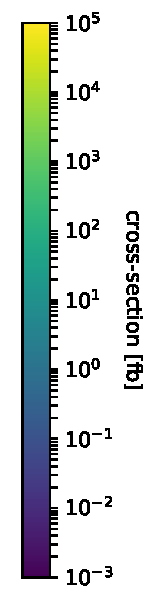
\includegraphics[height=3.5cm]{xsScans/3rdGen/cbar.pdf} %5000 fb\\
    \subfloat[$Y$ coupling to $u,d$ only]{\includegraphics[width=0.33\textwidth]{xsScans/1stGen/p_p____V_Y.pdf}} %5000 fb
    \subfloat[$Y$ coupling to $c,s$ only]{\includegraphics[width=0.33\textwidth]{xsScans/2ndGen/p_p____V_Y.pdf}} %5000 fb\\
    \subfloat[$Y$ coupling to $t,b$ only]{\includegraphics[width=0.33\textwidth]{xsScans/3rdGen/p_p____V_Y.pdf}} %5000 fb
    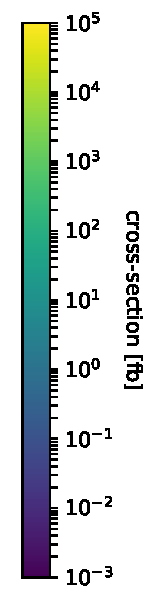
\includegraphics[height=3.5cm]{xsScans/3rdGen/cbar.pdf} %5000 fb
    \caption{Leading-order cross-sections extracted from Herwig for production of a $T$ and $Y$
      with a weak boson as a function of $M_Q$ and $\kappa$, for \SI{13}{\TeV} $pp$
      collisions, in the $\WZH = \WZHtoo$ scenario, assuming couplings to individual
      generations of quarks.  The white lines indicate the contours for production
      cross-sections in multiples of 10. First-generation couplings lead to higher
      production cross-sections, as a result of valence-quark-induced diagrams,
      while second and third-generation couplings lead to suppressed production
      rates, according to the relevant quark PDFs. Figure taken from Reference~\cite{VLQ_contur}.}
    \label{fig:QVproduction}
\end{figure}
Figures~\ref{fig:feyndiags}(\subref*{fig:feyndiags:Qq1}--\subref*{fig:feyndiags:Qq2}) show the single-production of VLQs in association with a quark, mediated by a weak boson. Considering the case where VLQs couple to first-generation quarks, the dominant production mechanism is the $t-$channel diagram where both the incoming quarks can be valence quarks. Diagrams with $dd$ induced VLQ production have the lowest cross-section, and $ud$ or $uu$ induced cross-sections are four times higher~\footnote{Since the proton composition is $uud$, the possible incoming quark pairs are: $uu, uu, ud,$; $uu, uu, ud,$; $du, du,$ and $dd$.}. Consequently, the dominant production process is $u + u \rightarrow X + q$, which is four times as frequent as the $dd$ induced $Y + q$. Both are mediated by a $W$ boson. For $B + q$ and $T + q$ production there is a further suppression from the small coupling of the Higgs boson to light SM quarks. When the VLQs couple to the second-generation quarks, the production cross-sections are dependent on the quark PDFs. For coupling to the third-generation, some production modes are inaccessible if they involve an incoming top quark. This effect is illustrated in Figure 4 of Reference~\cite{VLQ_contur} and reproduced in Figure~\ref{fig:Qqproduction}, where the production cross-sections for $T$ and $X$ in association with a quark are illustrated.
\begin{figure}[tbp]
    \vspace{-0.4cm}
    \subfloat[$T$ coupling to $u,d$ only]{\includegraphics[width=0.33\textwidth]{xsScans/1stGen/p_p____T_q.pdf}} %5000 fb
    \subfloat[$T$ coupling to $c,s$ only]{\includegraphics[width=0.33\textwidth]{xsScans/2ndGen/p_p____T_q.pdf}} %5000 fb\\
    \subfloat[$T$ coupling to $t,b$ only]{\includegraphics[width=0.33\textwidth]{xsScans/3rdGen/p_p____T_q.pdf}} %5000 fb
    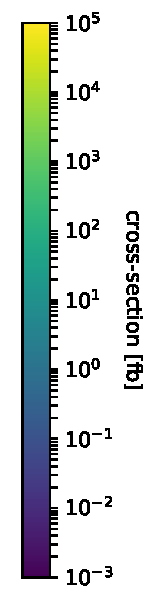
\includegraphics[height=3.5cm]{xsScans/3rdGen/cbar.pdf} %5000 fb \\
    \subfloat[$X$ coupling to $u,d$ only]{\includegraphics[width=0.33\textwidth]{xsScans/1stGen/p_p____X_q.pdf}} %5000 fb
    \subfloat[$X$ coupling to $c,s$ only]{\includegraphics[width=0.33\textwidth]{xsScans/2ndGen/p_p____X_q.pdf}} %5000 fb\\
    \subfloat[$X$ coupling to $t,b$ only]{\includegraphics[width=0.33\textwidth]{xsScans/3rdGen/p_p____X_q.pdf}} %5000 fb
    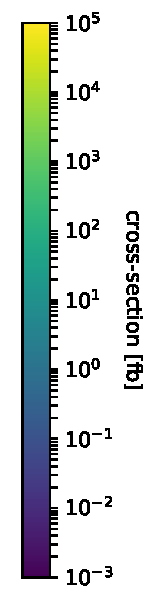
\includegraphics[height=3.5cm]{xsScans/3rdGen/cbar.pdf} %5000 fb
    \caption{Leading-order cross-sections extracted from Herwig for production of a $T$ and $X$
      with a SM quark as a function of $M_Q$ and $\kappa$, for \SI{13}{\TeV} $pp$
      collisions, in the $\WZH = \WZHtoo$ scenario, assuming couplings to individual
      generations of quarks.  The white lines indicate the contours for production
      cross-sections in multiples of 10. First-generation couplings lead to higher
      production cross-sections, as a result of valence-quark-induced diagrams,
      while second and third-generation couplings lead to suppressed production
      rates, according to the relevant quark PDFs. $X+q$ production goes from being
      the dominant production process at the LHC if $X$ couples to first-generation
      quarks only, to vanishing if $X$ couples to third-generation quarks only.
      White cells indicate corners of phase-space where the process in question is highly subdominant, and therefore where the cross-section was not sampled during the Herwig run. Figure taken from Reference~\cite{VLQ_contur}.}
    \label{fig:Qqproduction}
\end{figure}

\subsection{Comparison to \ATLAS searches}
Typically, searches conducted by the \ATLAS and \CMS experiments focus on the $T$ and $B$ vector-like quarks that couple only with the third generation SM quarks. In this sub-section the same assumption are made in order to compare the exclusions from \LHC results to exclusions computed by \contur. The $B$ and $T$ quarks are studied separately with all other VLQs decoupled from the SM. The possible decay channels are $b + Z$, $b + H$ and $t + W$ for the $B$ quark, and similarly $t + Z$, $t + H$ and $b = W$ for the $T$. Both \ATLAS and \CMS have conducted searches targeting specific final states~\todo{Provide some paper citations?}. \ATLAS published a combination limit from multiple searches of pair-produced VLQs in Reference~\cite{ATLAS_VLQ_combination}, and similarly from \CMS in Reference~\cite{Sirunyan_2018}. The \ATLAS results presents the exclusion limits in a two-dimensional parameter space of the VLQ branching ratios which is easily mimicked by \contur.

\begin{figure}[tbp]
    \vspace{-0.4cm}
    \subfloat[]{\includegraphics[width=0.45\textwidth]{B/1200/combinedOverlay}\label{fig:BTonlyB}}
    \subfloat[]{\includegraphics[width=0.45\textwidth]{T/1350/combinedOverlay}\label{fig:BTonlyT}}
    \caption{Sensitivity of LHC measurements to
    \protect\subref{fig:BTonlyB}~$B$-production for $M_B = \SI{1200}{\GeV}$ and
    \protect\subref{fig:BTonlyT}~$T$-production for $M_T = \SI{1350}{\GeV}$.
    The \contur exclusion is shown in the bins in which it is evaluated,
    graduated from yellow through green to black on a linear scale, with the 95\%~CL (solid white)
    and 68\%~CL (dashed white) exclusion contours superimposed. The mauve region
    is excluded at 95\%~CL by the ATLAS combination~\cite{Aaboud:2018pii}.}
    \label{fig:BTonly}
\end{figure}

Figure~\ref{fig:BTonlyB} shows the \contur exclusion region, in the half-plane
of different branching ratios, for $M_B = \SI{1200}{\GeV}$. This mass places it
in middle of the exclusion from ATLAS, which ranges from
\SIrange{1040}{1350}{\GeV} over the half-plane. The mauve region shows the
exclusion limit at 95\% confidence level (CL) by ATLAS. There are four main searches contributing to this limit, one each targeting the $Z$ and $H$ decay
channels~\cite{ZllSearch,HadSearch}, and the remaining two target $B$-decay to
$Wt$~\cite{WtSearch,TriLepSearch}. This results in a high sensitivity in the bottom-right
corner of the triangle, where $BR(B\rightarrow tW)$ is high. The sensitivity in
the measurements is somewhat complementary to the searches, and comes primarily
from $Z+$jet measurements~\cite{Aad:2015auj,Aaboud:2017hox,Aaboud:2017hbk,Aaboud:2019jcc}.

Figure~\ref{fig:BTonlyT} shows the \contur exclusion region for
$M_T = \SI{1350}{\GeV}$.  The ATLAS search exclusion for this mass value is also shown; in
this case, the ATLAS exclusion ranges from \SIrange{1310}{1420}{\GeV} over the
branching ratio half-plane. Here the difference in sensitivity between the ATLAS searches and \contur is nicely seen. From \contur, the exclusion comes primarily from measurements involving top quarks and $W$ bosons~\cite{Aaboud:2017fye,Aaboud:2018eqg,Sirunyan:2018wem,Khachatryan:2016mnb,Sirunyan:2018ptc}. The ATLAS combination limit in mauve on the other hand, has three contributions from searches sensitive to $T$-decay to $Ht$~\cite{HbbSearch,TriLepSearch,HadSearch}, two that target $T$-decay to $Zt$~\cite{ZnunuSearch,ZllSearch}, and only one sensitive in the $W$ channel~\cite{WbSearch}. Again, the measurement sensitivity is quite complementary to the searches.

\subsection{All quark generations}
% Although experimental searches assume that new quarks only couple to third generation SM quarks; mixings with lighter generations are not at all forbidden, and they can provide different signatures or affect the number of events in the final states tested by experiments, thus modifying current bounds.